\chapter{ Related Work }
\label{ssec:Related Work}

% \section{ Audio Plugin Standards }

\section{ Single-source, Multi-target Audio DSP }
"Write once, run anywhere" development and deployment of audio DSP algorithms is not a fundamentally new concept. Many solutions have arisen within the audio developer community, although none boast the advantages of a universal distributable.

% \vspace{24pt}

One approach is the use of \textit{intermediary plugin frameworks}, which have become very popular among audio developers\cite{2018_13}. Plugin frameworks provide a uniform application programming interface (API) in a particular programming language (typically C/C++) for producing many platform-specific executables from the same source code. The most widely used of these frameworks is JUCE\cite{JUCE}, which has become the industry standard. JUCE provides a C++ API by which the same audio processing and user interface code can be compiled for multiple targets, including cross-platform standalone applications, myriad plugin formats for digital audio workstations (DAWs), game engine plugins, and mobile apps. An alternative intermediary plugin framework, iPlug2\cite{2018_13}, adds Web Audio as a target via the Web Audio Modules\cite{10.1145/3487553.3524225} standard but is also implemented as a C++ API. Although both JUCE and iPlug2 provide the ability to address multiple targets from a single codebase, they still require separate compilation and binary distribution for each platform.

Another approach can be observed in the use of domain-specific languages (DSLs) for audio programming. Textual examples include CSound\cite{lazzarini2016csound}, FAUST\cite{orlarey:hal-02159014}, and CMajor\cite{huangc}; visual examples include Max\cite{MaxMSP8}, Gen\textasciitilde\cite{wakefield2012real}, and PureData\cite{puckette_puredata_1997}. The primary advantages of these languages are that they enable the developer to focus strictly on audio processing logic without handling memory management and other low-level programming tasks, and that they often target multiple deployments by exporting generated code. Some downsides are that they require programmers to learn a new language, that they may constrain the developer to a particular paradigm of signal processing, and that some are not free or open-source.

The ability of DSLs and intermediary plugin frameworks to target multiple deployment environments can be visualized as seen in Figure~\ref{fig1}. They are single-input, multiple output systems.

\vspace{12pt}

\begin{figure}[ht]
\centering
% \vspace{18pt}
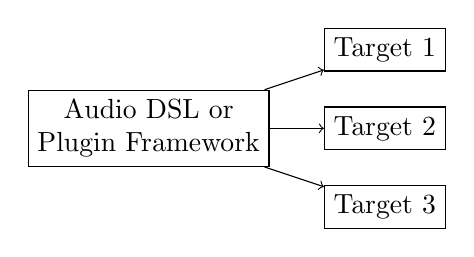
\begin{tikzpicture}
\node[draw,rectangle,align=center] (dsl) at (0,0) {Audio DSL or\\Plugin Framework};
\node[draw,rectangle] (t1) at (3,1) {Target 1};
\node[draw,rectangle] (t2) at (3,0) {Target 2};
\node[draw,rectangle] (t3) at (3,-1) {Target 3};
\draw[->] (dsl) -- (t1);
\draw[->] (dsl) -- (t2);
\draw[->] (dsl) -- (t3);
\end{tikzpicture}
\caption{\label{fig1}{\it Schematic representation of an audio DSL or plugin framework targeting multiple deployment environments.}}
\end{figure}

\begin{figure}[H]
\centering
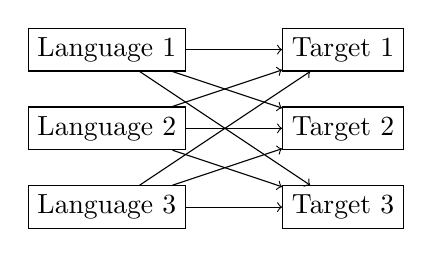
\begin{tikzpicture}
\node[draw,rectangle] (l1) at (0,1) {Language 1};
\node[draw,rectangle] (l2) at (0,0) {Language 2};
\node[draw,rectangle] (l3) at (0,-1) {Language 3};
\node[draw,rectangle] (t1) at (3,1) {Target 1};
\node[draw,rectangle] (t2) at (3,0) {Target 2};
\node[draw,rectangle] (t3) at (3,-1) {Target 3};
\foreach \i in {1,2,3} {
\foreach \j in {1,2,3} {
\draw[->] (l\i) -- (t\j);
}
}
\end{tikzpicture}
\caption{\label{fig2}{\it Schematic representation
of per-language, per-target toolchains.}}
\end{figure}

\begin{figure}[H]
\center
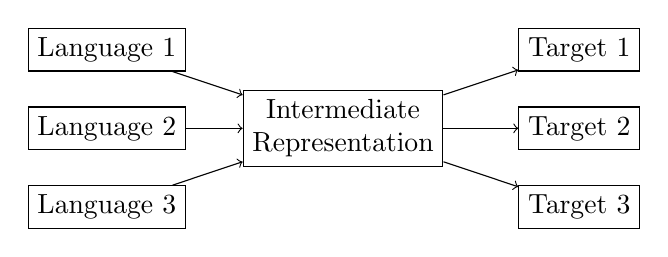
\begin{tikzpicture}
\node[draw,rectangle] (l1) at (0,1) {Language 1};
\node[draw,rectangle] (l2) at (0,0) {Language 2};
\node[draw,rectangle] (l3) at (0,-1) {Language 3};
\node[draw,rectangle,align=center] (ir) at (3,0){Intermediate\\Representation};
\node[draw,rectangle] (t1) at (6,1) {Target 1};
\node[draw,rectangle] (t2) at (6,0) {Target 2};
\node[draw,rectangle] (t3) at (6,-1) {Target 3};
\draw[->] (l1) -- (ir);
\draw[->] (l2) -- (ir);
\draw[->] (l3) -- (ir);
\draw[->] (ir) -- (t1);
\draw[->] (ir) -- (t2);
\draw[->] (ir) -- (t3);
\end{tikzpicture}
\caption{\label{fig3}{\it Schematic representation of multiple languages targeting an intermediate representation that supports multiple deployments.}}
\end{figure}

% \vspace{24pt}
\vspace{12pt}

A more flexible approach is a solution that can receive input in the form of source code from myriad programming languages, and also target multiple deployment environments. Traditionally, this may look like Figure~\ref{fig2}, which depicts how each programming language must have its own toolchain to target each deployment environment.

Using an intermediate representation, the complexity of a multi-input, multi-output system may be reduced. A runtime for the intermediate format in any deployment environment enables all programming languages that target the format to immediately target that deployment. In turn, any programming language that can compile to the representation is able to target any environment that supports a suitable runtime. This is visualized in Figure~\ref{fig3}.

\section{ WebAssembly in IoT Development }

The rapid growth of the Internet of Things (IoT) has intensified the need for development models that decouple application logic from hardware-specific implementation details\cite{PATEL201562}. Like the world of embedded audio, IoT deployments are characterized by extreme heterogeneity: devices vary widely in processor architecture, memory constraints, operating systems, and peripheral configurations. Traditionally, this diversity has required application developers to maintain separate codebases or heavily conditional builds for each target, increasing complexity and reducing portability.

To enable easier development and maintain of IoT software, streamlined multi-target development paradigms have emerged. These approaches enable software components written in different programming languages or otherwise originating from different toolchains (multi-source) to be deployed across diverse hardware platforms (multi-target) with minimal modification. Central to this model is the use of intermediate representation (IR), virtual execution layers, or other means that abstract away underlying architectural details. By targeting an IR, developers can focus on application logic and offload platform-specific implementation details to runtimes or translation layers designed to deterministically handle final deployment from a portable distributable.

WebAssembly (WASM) has gained attention in IoT research as such a portable, flexible IR\cite{10.1007/978-3-030-74296-6_27}\cite{10.1145/3593434.3593454}\cite{Rusum_2022}. Its well-defined execution semantics and compact binary format make it suitable for constrained devices, and toolchains exist to produce WASM from multiple source languages, including C/C++, Go, and Rust, enabling language-agnostic development. On the target side, WASM modules can be interpreted, just-in-time (JIT) compiled, or ahead-of-time (AOT) translated to native code, offering flexibility in runtime architecture.

This multi-source, multi-target model leveraging WASM reduces duplication of effort, improves maintainability, and enables modular software distribution across heterogeneous embedded systems. Its application to real-time audio DSP extends these principles to a domain with strict latency and determinism requirements, where portability has historically been limited by tight coupling between algorithms and hardware-specific toolchains.

% This work bridges two existing areas of research. In audio DSP, cross-platform development tools such as iPlug2 and FAUST have demonstrated the value of single-source, multi-target development. In parallel, Internet of Things (IoT) research has investigated WebAssembly as a secure, portable "write once, run anywhere" substrate for sandboxed applications. Combining these trajectories, this study evaluates WebAssembly as a distribution format for encapsulated audio DSP modules.

\section{ Existing Approaches to Third-Party Plugins in Embedded Audio}

Third-party plugins for embedded audio systems have been explored in industry, hobbyist and research contexts, but mass adoption is yet to occur.

One approach is use of the LV2 audio plugin standard, a format specific to Linux. A major advantage of using LV2 is that it is available as a JUCE target, so existing JUCE plugins can be ported to new Linux platforms with a conditional build for the host architecture. Some downsides of this approach are that an operating system is required, and that most existing JUCE plugins do not have graphical user interfaces (GUIs) tailored to embedded systems. Examples that use the LV2 approach such as the MOD Audio ecosystem\cite{mod_audio_platform} and Darkglass Anagram\cite{darkglass_plugin_dev_setup} encourage plugin developers to make custom GUIs for each platform.

\begin{figure}[ht]
\vspace{12pt}
\centerline{
\includegraphics[scale=0.1]{LPA-Paper/figures/ana.pdf}}
\caption{\label{fft_plot}{\it The Darkglass Anagram, a commercial product that supports LV2 plugins }}
\end{figure}

An issue facing systems that depend on LV2 is that users are beholden to developers of their favorite plugins to produce and publish binaries targeting their particular hardware, and most vendors of popular audio plugins do not publish LV2 binaries.  A unique approach for porting commercial plugins to Linux systems that bypasses this problem can be studied in \cite{interfacinglinux_yabridge}. Using \lstinline{yabridge}\cite{yabridge_repo}, a compatibility layer for running Windows audio plugin binaries on Linux, this hobbyist demonstrated how popular VST plugins can be used on Linux systems. The major disadvantage is that performance degradation was shown to be ~50\%. They did not explicitly demonstrate Windows VSTs running on \textit{embedded} Linux, but the primary problem of adapting user interface by connecting to a remote GUI or physical controls could be resolved in the implementation of the plugin host.

Another approach is one presented by researchers in \cite{spittle2021developing}, who implemented a novel framework for developing embedded audio applications that expect the GUI and audio processing to be separated over network. This approach relies on a custom operating system they maintain, called EarOS.

While not explicitly related to plugins, researchers in \cite{lai2025audioreach} developed an open-source framework for deploying the same audio processing to heterogeneous embedded systems. Their support for third-party audio processing defined in C or MATLAB/Simulink provides an example of coexistence between embedded audio modules authored in different programming languages.

% Sonical
% AudioReach
% BeagleBone
